% !TeX root = solutions_main.tex

\section*{Solution 2: Stick Slip (Filippov Behaviour)}
\begin{enumerate}[label=\alph*)]
\item \textbf{Right-hand side} 
\newline
File name: \texttt{rhsTask2Fil.m}
\begin{lstlisting}
function dx = rhsTask2Fil(t, x, p)
% p = (k, m, v_b, F_s, delta, epsilon)
k       = p(1);
m       = p(2);
v_b     = p(3);
F_s     = p(4);
delta   = p(5);
epsilon = p(6);
v_rel   = x(2) - v_b;

dx = zeros(2,1);
dx(1) = x(2);

dx(2) = -(k / m) * x(1) + F_fil(v_rel, F_s, delta) / m;
end
\end{lstlisting}
File name: \texttt{F\_fil.m}
\begin{lstlisting}
function res = F_fil(v_rel, F_s, delta)
  if v_rel <= 0
    res = F_s / (1 - delta * v_rel);
  end
  if v_rel > 0
    res = -F_s / (1 + delta * v_rel);
  end
end
\end{lstlisting}

\noindent
Now, the main executable file can be modified and called. Here shown are only the relevant sections. Find the full \texttt{.m} file in the Heibox:
File name: \texttt{runTask2.m}
\begin{lstlisting}
% ...
%% Model setup
tspan = [0, 30];
y0 = [1; 0];
k       = 1.0;      % spring constant
m       = 1.0;      % mass
v_b     = 0.2;      % velocity relative to the conveyerbelt
F_s     = 1.0;      % max static friction force
delta   = 3.0;      % Physics constant
epsilon = 1e-10;    % numerical zero parameter
p = [k, m, v_b, F_s, delta, epsilon];

% ...

%% Solving the friction model variant with sliding mode
slidingRhs = @rhsTask2Fil;
slidingDatahandle = prepareDatahandleForIntegration(slidingRhs,... 
	'integrator', integrator,... 
	'options', optionsOde);
slidingSol = solveODE(slidingDatahandle, tspan, y0, p);

%% Plot solution for model with sliding mode
plotSolution(slidingSol, ...
	'tplot', tplot, ...
	'title', 'ODE Solution to Friction Model (Sliding Mode)', ...
	'legend', legendSol);
\end{lstlisting}

\item As expected, the system shows periodic behaviour of which the "Stick" phase shows Filippov chattering. These regions are the marked ones in the plot on the exercise sheet.

\item The RHS function is the following:\\
File name: \texttt{rhsTask2noFil.m}
\begin{lstlisting}
function dx = rhsTask2noFil(t, x, p)
% p = (k, m, mu_b, F_s, delta, epsilon)
k       = p(1);
m       = p(2);
mu_b    = p(3);
F_s     = p(4);
delta   = p(5);
epsilon = p(6);
mu_rel  = x(2) - mu_b;

dx = zeros(2,1);
dx(1) = x(2);
dx(2) = -(k / m) * x(1) + F_noFil(x, mu_rel, epsilon, F_s, k, delta) / m;

end
\end{lstlisting}
with a formulation of the intrinsic function using reduced branching\\
File name: \texttt{F\_noFil.m}
\begin{lstlisting}
function res = F_noFil(x, mu_rel, epsilon, F_s, k, delta)
  if mu_rel <= -epsilon
    res = F_s / (1 - delta * mu_rel);
  else
    if mu_rel >= epsilon
      res = (-F_s) / (1 + delta * mu_rel);
    else
      if k*x(1) <= -F_s
        res = F_s;
      else
        if k*x(1) >= F_s
          res = F_s;
        else
          res = k*x(1);
        end
      end
    end
  end
end
\end{lstlisting}

\noindent
Now as before, the relevant parts from \texttt{runTask2.m}
\begin{lstlisting}
%% Solving the friction model variant without sliding mode
noSlidingRhs = @rhsTask2noFil;
noSlidingDatahandle = prepareDatahandleForIntegration(noSlidingRhs, 'integrator', integrator, 'options', optionsOde);
noSlidingSol = solveODE(noSlidingDatahandle, tspan, y0, p);

%% Plot solution for model without sliding mode
plotSolution(noSlidingSol, ...
	'tplot', tplot, ...
	'title', 'ODE Solution to Friction Model', ...
	'legend', legendSol);
\end{lstlisting}
\end{enumerate}

Here are the plots of all variants including the difference plot:
\begin{figure}[H]
	\centering
	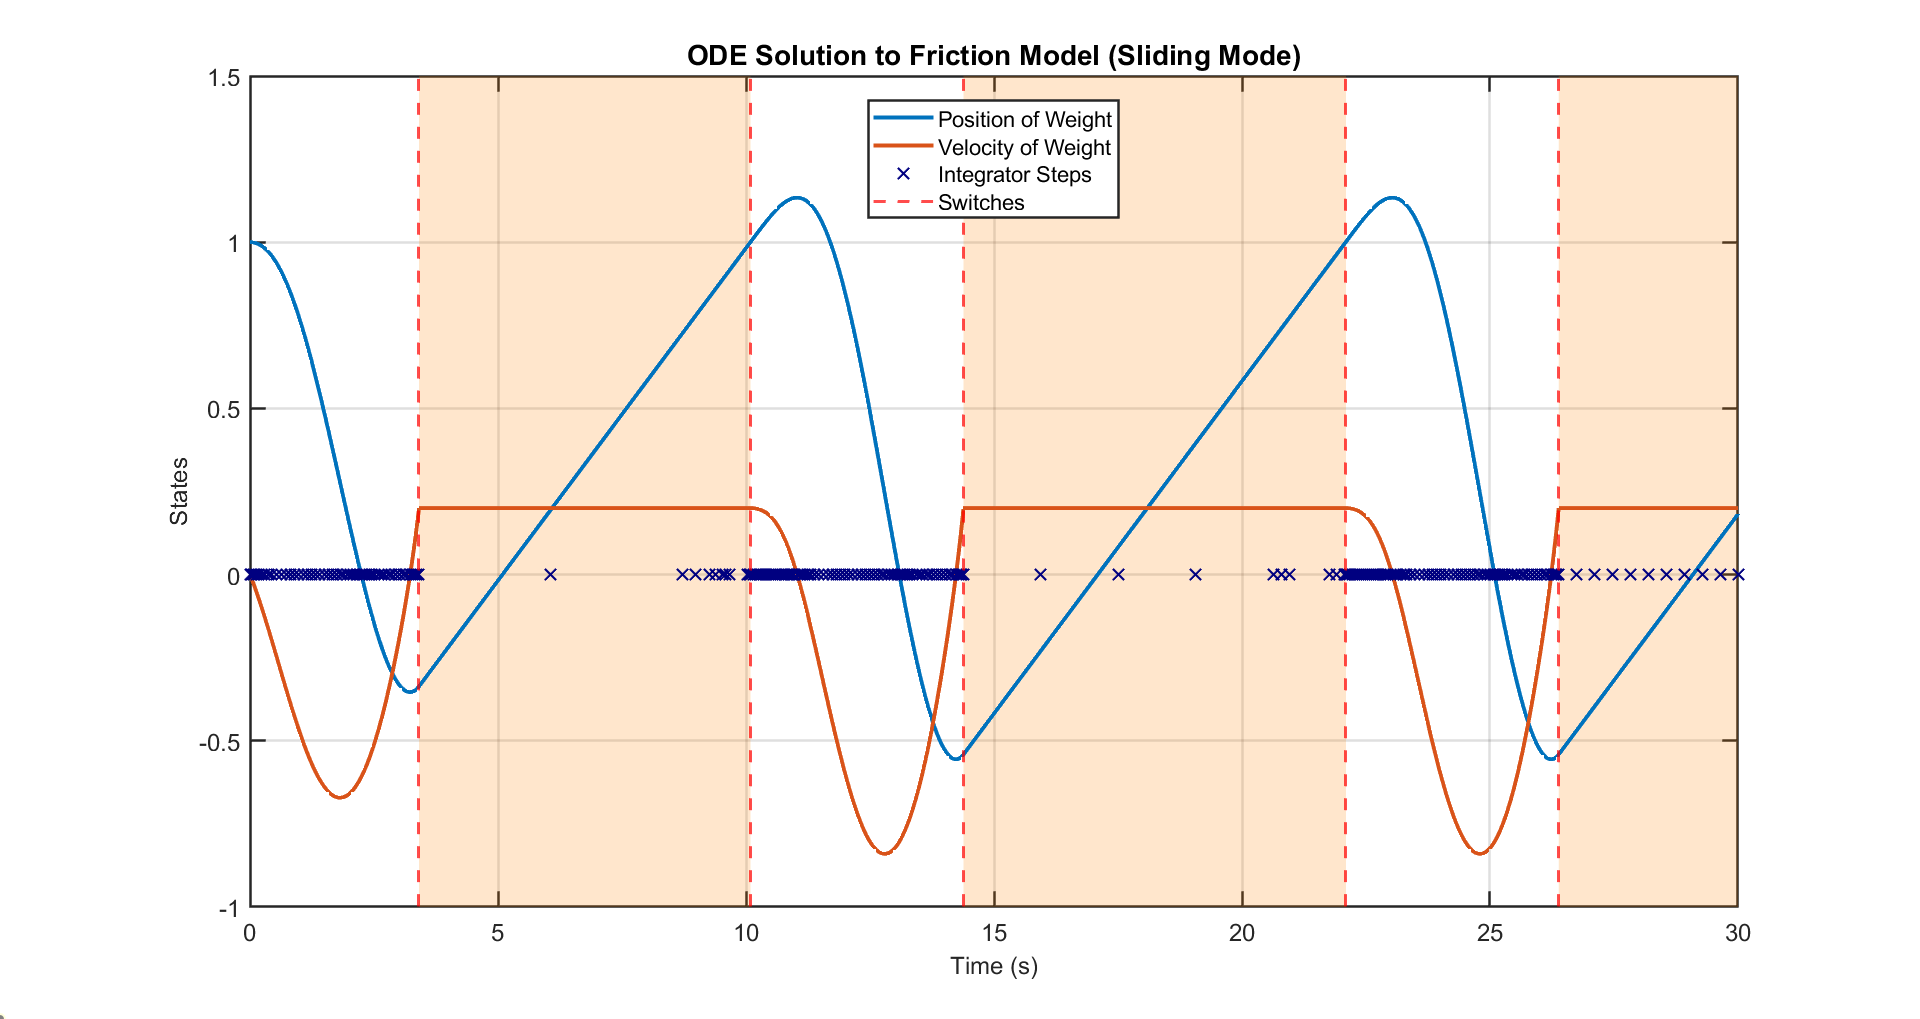
\includegraphics[width=1\linewidth]{Plots/task2a.png}
	\caption{Solution using Filippov mode of IFDIFF}
\end{figure}
\begin{figure}[H]
	\centering
	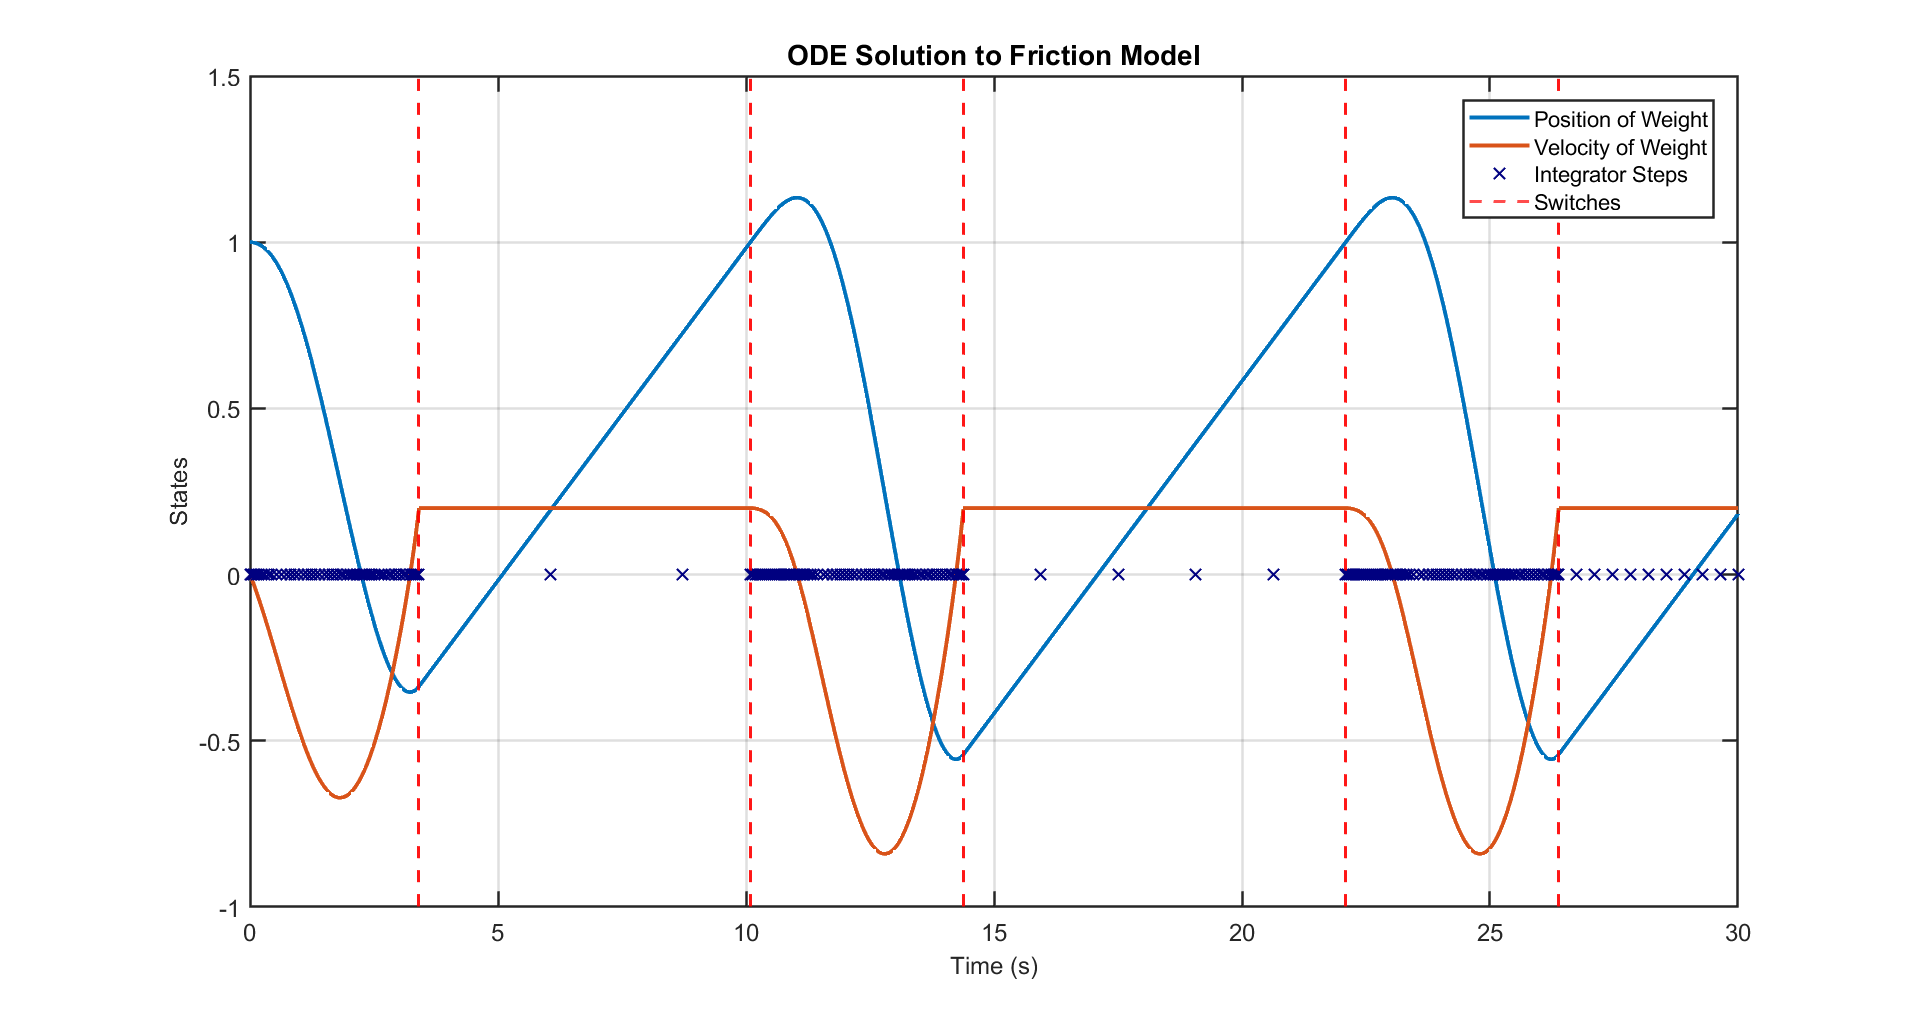
\includegraphics[width=1\linewidth]{Plots/task2c.png}
	\caption{Reference solution, using the more complicated RHS formulation}
\end{figure}
\begin{figure}[H]
	\centering
	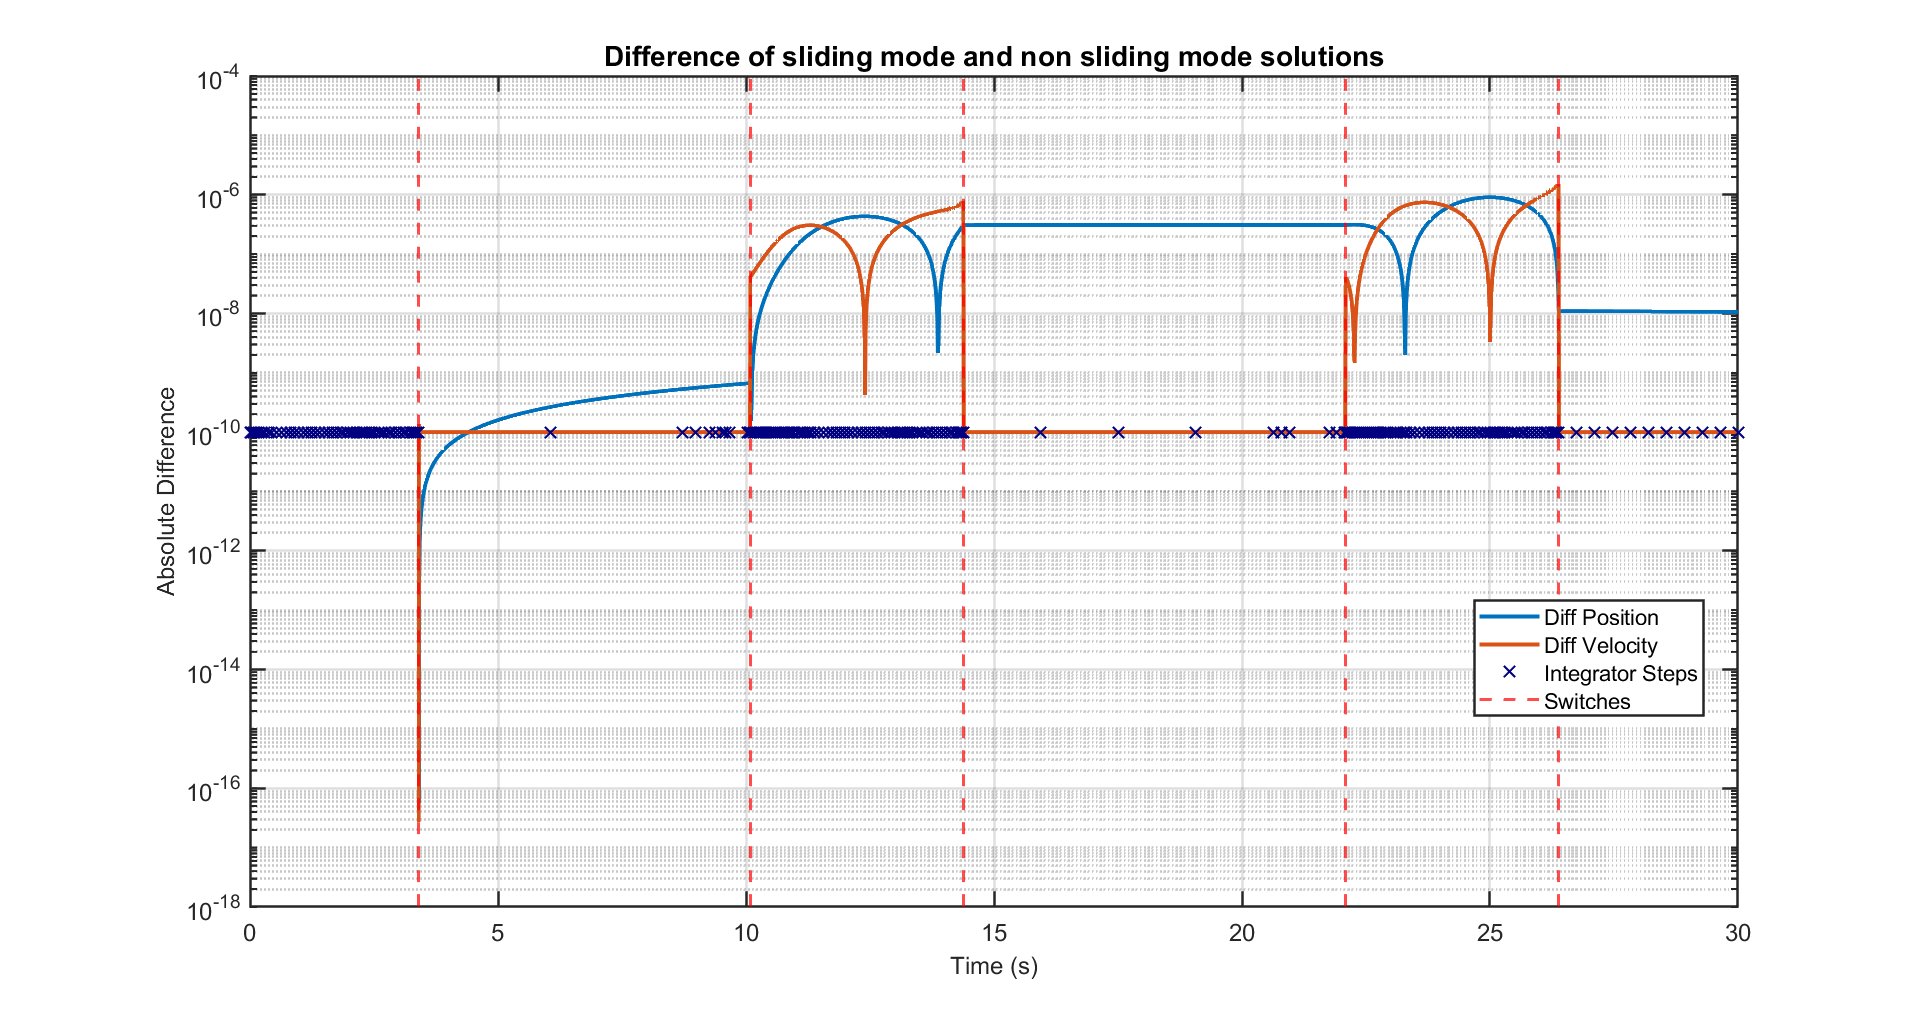
\includegraphics[width=1\linewidth]{Plots/task2_diff_plot.png}
	\caption{Difference Plot}
\end{figure}

